%%% PRomemoria, 20 pagine


% Chapter results

\chapter{Results achieved by the Candidate} % Main chapter title

\label{Chapter5} % For referencing the chapter elsewhere, use \ref{Chapter4} 

%----------------------------------------------------------------------------------------



%~~~~~~~~~~~~~~~~~~~~~~~~~~~~~~~~~~~~~~~~~~~~~~~~~~~~~~~~~~~~~~~~~~~~~~~~~~~~~~~~~~~~~~~


%%%%%%%%%%%%%%%%%%%%%%%%%%%%%%%%%%%%%%%%%%%%%%%%%%%%%%%%%%%%%%%%%%%%%%%%%%%%%%%%%%%%%%%
%  Section 
%%%%%%%%%%%%%%%%%%%%%%%%%%%%%%%%%%%%%%%%%%%%%%%%%%%%%%%%%%%%%%%%%%%%%%%%%%%%%%%%%%%%%%%

%\section{Description vgpop}
\section{Implementation of the \vgp library}  

I developed a library named \vgp to conduct standard population genetics analyses using pangenomic data models. Typically represented in the Graphical Fragment Assembly (GFA) format, these models can represent whole genome alignments in a compact graphical structure. The library is written in Python programming language under MIT license; the code is publicly available on GitHub (\url{https://github.com/Flavia95/VGpop}) 

At its present state \vgp contains seven functions briefly introduced in tab \ref{tab:functionvgpop} and detailed in the following paragraphs.

%\vspace{1cm}

{\small
\begin{table}[H]
\caption{Functions implemented in \vgp}
\label{tab:functionvgpop}
\centering
\begin{adjustbox}{width=0.80\textwidth}
\begin{tabular}{c c c c }
\toprule
\tabhead{vgpopfunction} & \tabhead{Description} & Input & Output \\
\midrule
bubblepop & Identification of polymorphic genomic regions (bubbles) &  GFA & dictionary  \\
bubblecall & variant calling and positioning  &  dictionary & dictionary  \\
gfa2vcf & Conversion of files in GFA format to VCF format & GFA & VCF \\
gfa2allelefreq & Calculation of allele frequencies & GFA & allelefreqfile \\
gfa2genofreq & Calculation of genotype frequencies & GFA & genotypefrequenciesfile \\
gfa2fst & Calculation of F\textsubscript{ST} & GFA & fstfile\\
seqgen2gfa+vcf & File conversion from Seq-Gen & Seq-Gen & GFA, VCF \\
\bottomrule\\
\end{tabular}
\end{adjustbox}
\end{table}
}

%\vspace{1cm}

%%%%%%%%%%%%%%%%%%%%%%%%%%%%%%%%%%%%%%%%%%%%%%%%%%%%%%%%%%%%%%%%%%%%%%%%%%%%%%%%%%%%%%%%%%%%
%  Subsection 
%%%%%%%%%%%%%%%%%%%%%%%%%%%%%%%%%%%%%%%%%%%%%%%%%%%%%%%%%%%%%%%%%%%%%%%%%%%%%%%%%%%%%%%%%%%%


\subsection{\bbp}

The main challenge of my project was to extract the information about variable sites (i.e. regions where more that one type of sequence is present) from the graphs. Any population genetic analysis is indeed based on the information contained in the variable segments of the sequence and their occurrence in the population under investigation. Because of their appearance in the pangenome graph, variable sites are referred to as bubbles (Figure \ref{fig:gfa.png}). 

The core of \vgp is the \bbp function, which takes as input a pangenome, detects bubbles, and outputs the sequences of the variants contained in the bubbles.

The code I developed for the \bbp function takes as input a GFA file and gives as output a dictionary, i.e. a table of correspondences between region of the graph and sequence variants. It explores the graph using the two recursive algorithms described in the following paragraphs and works in two consecutive steps. 

%% non servono le lettere, zzom dalontano, graph piu' complesso senza dettaglio si fa vdere DFS sceglie un nodo  eesplora a casa un pezzoee  
%tree con root piu' lontana, aggiungere un pezzo di root 

\begin{figure}[H]
\centering
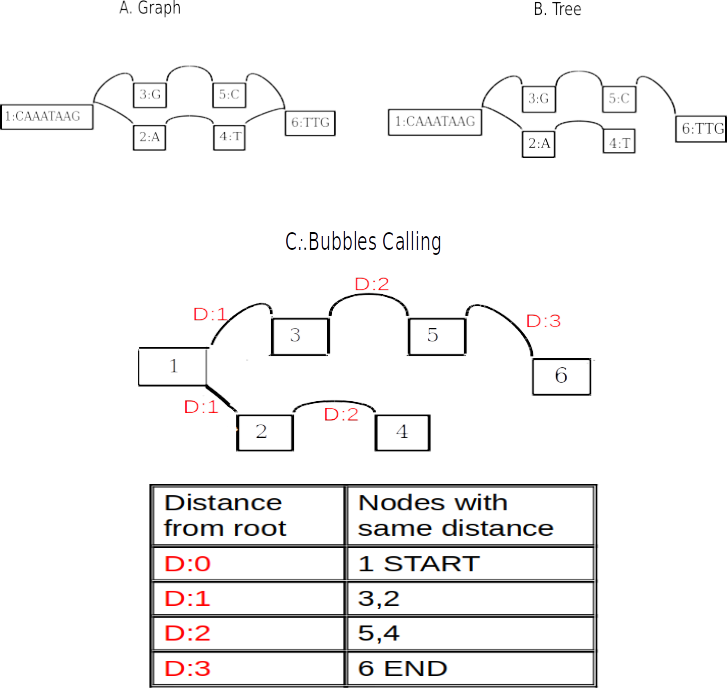
\includegraphics[width=1.00\textwidth]{fig/bubblepop.png}
\decoRule
\caption{\textit{bubblepop} transforms a pangenome (\textbf{A}) in a tree (\textbf{B}) using two algorithms, the Depth First Search and the Breadth first Search. On tree identify bubble (\textbf{C})}
\label{fig:bubblepop.png}
\end{figure}


\setcounter{secnumdepth}{3}
\subsubsection{Step 1: Depth first Search}

%I use two recursive algorith \cite{geeksforgeeks.org}.%questo e' un sito generico
The Depth First Search (DFS) \cite{korf1985depth,wiki:DFS} is a recursive algorithm for searching graph data structures. DFS select an arbitrary node as root node and explores as far as possible along each branch. The exploration process runs until some depth cutoff is reached, and then DFS backtracks to the next most recently expanded node. Therefore, only the path of nodes from the initial  node to the current  node  must be stored in order to execute the algorithm (Figure \ref{fig:bubblepop.png}A). At each iteration, DFS marks each node of a graph as visited and piles it up on a stack of visited nodes. \\

In \bbp I use the DFS algorithm to explore the graph starting from a random node of the pangenome. At each iteration, \bbp creates a spanning tree from the part of the pangenome that is explored (Figure \ref{fig:bubblepop.png}B), threfore transforming the pangenome in a trees. In trees obtained from pangenomes, the branches are obtained by resolving the bubble into its edges components and the nodes represent chunks of sequences.  

\subsubsection{Step 2: Breadth first Search}
Breadth First Search (BFS) \cite{beamer2012direction,programiz.com}, is another recursive algorithm for traversing or searching tree or graph data structures. I used BFS on the tree obtained applying DFS (Figure \ref{fig:bubblepop.png}B). When used on trees, at each iteration BFS starts at the tree root and explores all of the neighbor nodes at one step, then expands to the nodes at the next steps until a goal state is reached \cite{korf1985depth, wiki:BFS}. The information encountered during the exploration is recorded and the nodes that are visited are marked.\\  
 
In \bbp, I used BFS on the tree obtained by DFS (Figure \ref{fig:bubblepop.png}B). Starting from the tree root DFS explores the tree until it finds a bubble. When this happens it calculates the distance from the root of all the nodes in the bubbles and stores this information in a dictionary, i.e. a table of correspondence (Figure \ref{fig:bubblepop.png}). 

%AGGIUNGERE COME SI CONSERVANO I PATHS: non so se metterlo, sono già presenti nel grafo ma nella mia implementazione ho creato dizionari per comodità ma si dovrebbe sfruttare che sono nel GFA.odgi. 

\subsection{\bbc}
Once the pangenome has been decomposed with \bbp in a tree whose information on the node distance from the root is stored in dictionary, \bbc make explicit the content of the bubbles and its position along a chosen reference sequence.    

Within the dictionary, the beginning and the end nodes of a bubbles are identified by the fact that their distance from the root is unique, i.e. they are the only nodes with a specific distance from the root (Figure \ref{fig:bubblepop.png}C). All other nodes are inner nodes of bubbles and correspond to variable regions of the sequence. Furthermore nodes with the same distance from the root are in the same bubble.\\

\noindent
The code I developed for \bbc works in three steps:

\begin{enumerate}
\item\textbf{Choice of the reference path}

Considering all the possible paths that connect the initial node and the final node of each bubble, I chose the first path in GFA file as reference (REF).

%Considering all the possible paths that connect the initial node and the final node of each bubble. I chose first path in GFA as reference (REF). I considered all the possible paths pairs(x,y) which x is the REF. I went through the bubbles and along the two paths I defined the variants.
 %Sono andata nelle bubble e percorrendo i due path ho definito le varianti, OK SPIEGATO % 
As implemented now, the first path in the GFA file is used as reference, however it is possible to set any available paths as reference.

\item\textbf{Variant identification} In this step \bbc iterates over all available nodes to compare them with the corresponding reference node, where the correspondence is defined by the flanking nodes (Figure \ref{fig:path_ref.png})
%quella di prima o questa di dopo? spostata qui perche' parla di varianti
I considered all the possible paths pairs(x,y) which x is the REF. I went through the bubbles and along the two paths I defined the variants.

A node is called as a variant if: 
\begin{itemize}
    \item (i) it is supported by at least one path; 
    \item (ii) the node sequence is different from the sequence of the corresponding reference node; 
    \item (iii) if its distance from the root is the same as the one of the reference node, than the variant is classified as a Single Nucleotide Variants (SNV)
    \item (iv) if its distance from the root is smaller that the one of the reference node then the variant is classified as a Deletion  
    \item (v) if its distance from the root is greater that the one of the reference node then the variant is classified as an Insertion
\end{itemize}

\item \textbf{Variant positioning} This step defines the position of a variants with respect to the reference sequence. When the two paths were used to call the variants, the length of the sequences was taken into account in order to map the variants on the individual paths.%Todo:spiegare, spiegato
\end{enumerate} 

%QUando sono stati percorsi i due path per chiamare le varianti, si è tenuto conto della lunghezza delle sequenze per poter mappare le varianti sui singoli path.Example POS, for example (NODE1 ATG) POS is 3 (length of sequence); for (NODE2 AT) POS is 5 because is the sum of the length of the previous node sequence plus the current node length sequence.

%aggiungere distance from root, tipo mettere root a sinistra e fare un asse con le distanze , tipo asse x 
%scrivere invece dei numeri n1, n2, n3, n4, etc.. (con i numeri che fanno al caso, ovviamente). potresti pur efare un circolo e mettere n1, dentro, sarebbe piu' chiaro  si potrebbe anche mettere un sequenza semplice 
\begin{figure}[H]
\centering
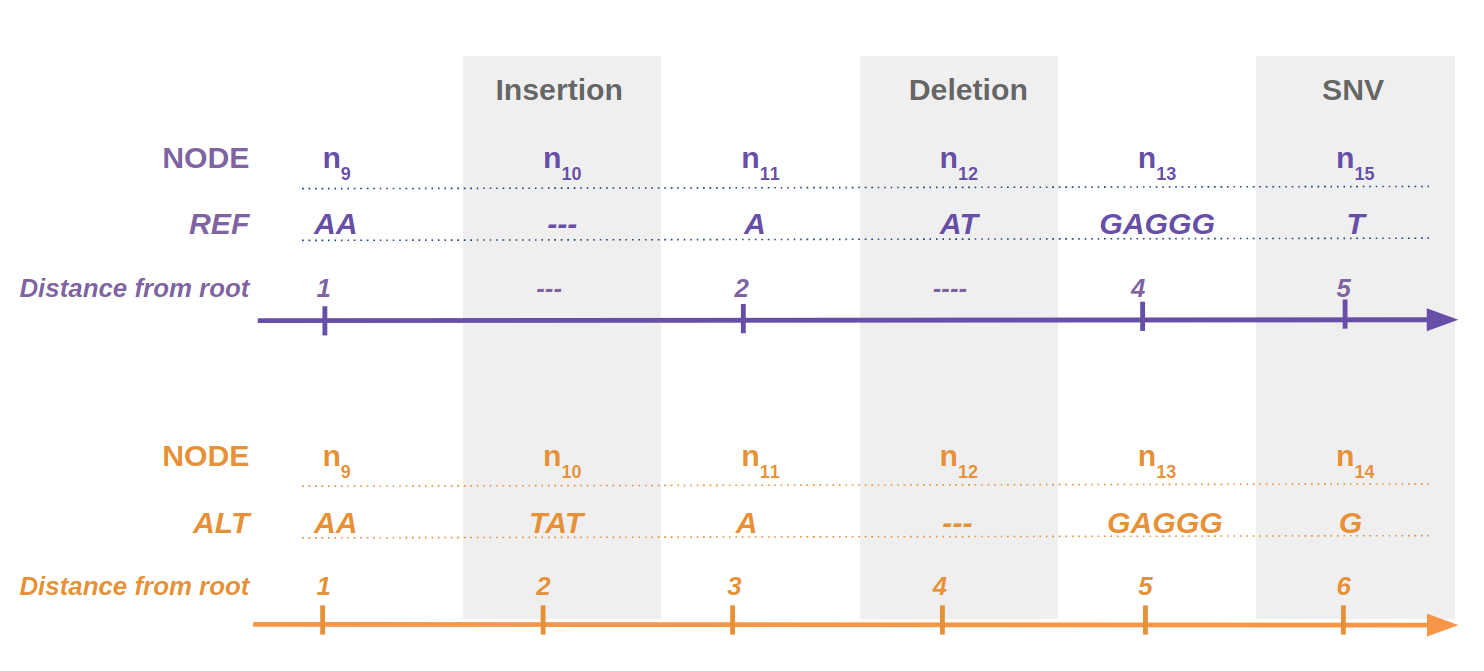
\includegraphics[width=1.00 \textwidth]{fig/path_ref.png}
\decoRule
\caption{\textbf{Variant identification by the \bbc function.} Nodes here are represented by their node names and sequences and their distance from the root is reported. A path is chosen as reference (REF) and used to iteration combination with all other possible paths. Within the iteration, nodes between paths (REF and the one under consideration) are compared. \\If a node in the path under consideration is present, has the same distance from root as REF, and is different from REF, then a \textbf{Single Nucleotide Variant (SNV)} is called. Instead, if a node in the path under consideration is not found in the REF, than the node distance from root is compared with the corresponding empty position on REF: an \textbf{Insertion} or a \textbf{Deletion} is called, according to if the node distance is greater or smaller, respectively.}
%\caption{Scheme of the output of \textit{bubblecall} function. The path used as REF and call variant in a path}
\label{fig:path_ref.png}
\end{figure}

%distanza root, sotto ognuno di ref e alt riga distanza root. 





%figura con A. figura bubble, B. tabella tipo vcf con indel ecc.  C same as A ma piu; complesso  D same as B 

%fare ora
\begin{figure}[H]
\centering
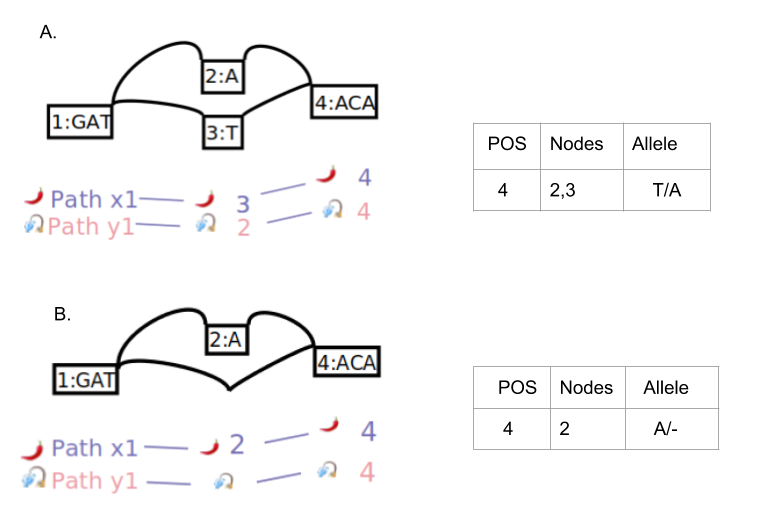
\includegraphics[width=1.00\textwidth]{fig/bubblesimpleandcomplex.png}
\decoRule
\caption{\textbf{Fig A: Bubble}. Path x represents the sequence used as a reference to describe variants that are present in a sequence analysed.} 
\label{fig:bubble.png}
\end{figure}


%I obtained VCF.

%%%%%%%%%%%%%%%%%%%%%%%%%%%%%%%%%%%%%%%%%%%%%%%%%%%%%%%%%%%%%%%%%%%%%%%%%%%%%%%%%%%%%%%%%%%%
%  Subsection 
%%%%%%%%%%%%%%%%%%%%%%%%%%%%%%%%%%%%%%%%%%%%%%%%%%%%%%%%%%%%%%%%%%%%%%%%%%%%%%%%%%%%%%%%%%%%

\setcounter{secnumdepth}{3}
\subsection{gfa2vcf}
%tolto the second, non c'e un ordine 
The code I developed for the \textit{gfa2vcf} function of \vgp takes as input a graph in the GFA format and output a corresponding linear representation in the VCF format. To do this \textit{gfa2vcf} uses first \bbp to decompose the pangenome in a tree and then \bbc to identify the variable sites. Finally the dictionary of the variable site is formatted according to the vcf specifications. 

{\small
\begin{table}
\caption{Correspondences between elements of the GFA and VCF}
\label{tab:gfatovcf}
\centering
\begin{adjustbox}{width=0.50\textwidth}
\begin{tabular}{c c}
\toprule
\tabhead{GFA} & \tabhead{VCF} \\
\midrule
 Path Name & CHROM \\
 Position in the reference sequence & POS \\
 Sequence of bubble's inner nodes & REF allele  \\
  that is present in the path chosen as reference  &  \\
 Sequence of bubble's inner nodes & ALT allele  \\
  that is NOT present in the path chosen as reference  &  \\
 SNV, INDEL & Type\\
\bottomrule\\
\end{tabular}
\end{adjustbox}
\end{table}
}

%non farei una sub sub section 
%\subsubsection{Validation of the VCF obtained with \textit{gfa2vcf}}
To validate the VCF obtaind using \textit{gfa2vcf}, I reconstructed a graph starting from it and using an existing tool, i.e. the functions \textit{vgconstruct} and \textit{vgview} from the \textsc{vgtool}  library \cite{vg,vgteam}) (Figure \ref{fig:validationgraph.png}A). The graph used as input of \textit{gfa2vcf} and the one reconstructed with \textsc{vgtool}, are identical, suggesting that the \textit{gfa2vcf} works well (Figure \ref{fig:validationgraph.png}B).  

%%cambiare GFA start con GFA from \vgp  e GFA con GFA from \textsc{vgtools} DIDALSCALIA GIA@ CAMBIATA , 

%per Enza, non mi trovo perchè GFAstart from vgpop??? E' un GFA costruito indipendentemente che poi trasformo in VCF
\begin{figure}[H]
\centering
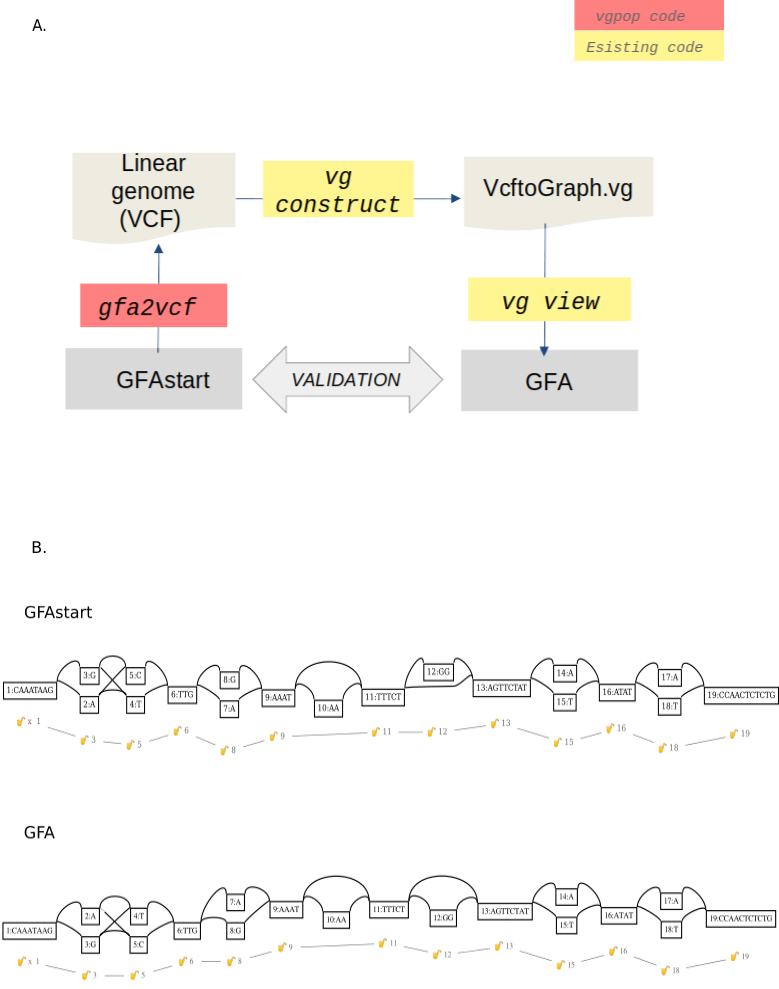
\includegraphics[width=0.80 \textwidth]{fig/validationgfa2.vcf.png}
\decoRule
\caption{Validation scheme of the \textit{gfa2vcf} function (\textbf{A}). the graph used as input from \vgp is identical to the one reconstructed using \textsc{vgtools} from the VCF obtained by \textit{gfa2vcf} (\textbf{B})}
\label{fig:validationgraph.png}
\end{figure}

%%%%%%%%%%%%%%%%%%%%%%%%%%%%%%%%%%%%%%%%%%%%%%%%%%%%%%%%%%%%%%%%%%%%%%%%%%%%%%%%%%%%%%%%%%%%
%  Subsection 
%%%%%%%%%%%%%%%%%%%%%%%%%%%%%%%%%%%%%%%%%%%%%%%%%%%%%%%%%%%%%%%%%%%%%%%%%%%%%%%%%%%%%%%%%%%%

\subsection{gfa2allelefreq} 

The \textbf{frequency of an allele} is an indication of how common the allele is in a population. It is calculated by counting how many times the allele appears in the population, dividing by the total number of copies of the gene.\\

For a locus with \emph{p} alleles, the allele frequency of the \emph{i\textsubscript{th}} allele \emph{p\textsubscript{i}} in a population of haploid individuals is: 

Haploid allele frequency    $p\textsubscript{i} = \dfrac{i}{N}$

\noindent
where \emph{i} is the count of the alleles and \emph{N} is the number of individuals in the population.\\
\noindent
In a diploid populations the formula becomes: 

Diploid allele frequency  $p\textsubscript{i} =  \dfrac{i}{2N}$\\

The code I developed for the \textit{gfa2allelefreq} function of \vgp takes as input a graph in GFA format and a metadata file (with information on paths, individuals, and populations), and outputs a file that contains the allele frequencies for variable loci per each population. In \textit{gfa2allelefreq} the allele frequency corresponds to the number of paths that support a node (i.e. a variant) divided by the total number of paths actually realized. The frequencies of monomorphic nodes (i.e. frequency = 1) are not reported.  %attenzione: riusciamo a discriminare i paths effettivamente realizzati da tutti quelli possibili? (considered even REF)
\textit{gfa2allelefreq} first uses \bbp and \bbc to read the graph, and than applies calculation of frequencies.

%In this specific case I obtained two file of calculation, one from each population. 

 %descrivere metadata, info individui e haplo
 

%%%%%%%%%%%%%%%%%%%%%%%%%%%%%%%%%%%%%%%%%%%%%%%%%%%%%%%%%%%%%%%%%%%%%%%%%%%%%%%%%%%%%%%%%%%%
%  Subsection 
%%%%%%%%%%%%%%%%%%%%%%%%%%%%%%%%%%%%%%%%%%%%%%%%%%%%%%%%%%%%%%%%%%%%%%%%%%%%%%%%%%%%%%%%%%%%
\subsection{gfa2genfreq}

The \texbf{frequencies of a genotype} in a population is the ratio between the count of individuals with a given genotype and the total number of individuals in the population. For haploid population genotypic frequencies coincide with allelic frequencies.  \cite{brooker2014principles}.
%GIA DETTO In population genetics, the genotype frequency is the frequency or proportion of genotypes in a population. 

%$f(a) = \dfrac{(Aa) + 2 x (aa))}{2 x (AA) + 2 x (Aa) + 2 x (aa)}$
For a locus with \emph{g} alleles in a population of diploid individuals, the number of possible genotypes is the sum of the integers between 1 and g. As an example, for a locus with 3 alleles. 1+2+3=6 genotypes are possible. The genotype frequency of the \emph{i\textsubscript{th}} genotypes \emph{g\textsubscript{i}} is: 

Genotype frequency    $g\textsubscript{i} = \dfrac{i}{2N}$\\

\noindent
where \emph{i} is the count of the individuals with genotype \emph{g\textsubscript{i}} and \emph{N} is the number of individuals in the population.\\

The code I developed for the \textit{gfa2genfreq} function of \vgp takes as input a graph in GFA format and a metadata file (with information on paths, individuals, and populations) and outputs a file that contains the genotype frequencies of all possible genotypes. In \textit{gfa2genofreq} \emph{2N} is the number of paths actually realized and for each genotype \emph{g\textsubscript{i}}, \emph{i} is determined using the information of the metadata. 
\textit{gfa2genfreq} first uses \bbp and \bbc to read the graph, and than applies calculation of genotypes.
%%%non cpaisco 
%I counted ATGC in a position and I checked the reference base and calculate for each allele the frequency (count/numhaplotype).


%%%%%%%%%%%%%%%%%%%%%%%%%%%%%%%%%%%%%%%%%%%%%%%%%%%%%%%%%%%%%%%%%%%%%%%%%%%%%%%%%%%%%%%%%%%%
%  Subsection 
%%%%%%%%%%%%%%%%%%%%%%%%%%%%%%%%%%%%%%%%%%%%%%%%%%%%%%%%%%%%%%%%%%%%%%%%%%%%%%%%%%%%%%%%%%%%


\subsection{gfa2fst}
%referenza wright fisher con calma
%metti figura da paper TIG 
The Wright’s fixation index ($F\textsubscript{st})$ is a measure of population differentiation due to genetic structure. It is estimated from genetic polymorphism data, such as SNV or microsatellites. Several formulae exists for its calculation among which the one that estimates it as the standardized variance of allele frequencies among sub-populations:\\

$F\textsubscript{st} = \dfrac{s^{2}}{p(1-p)}$\\

with \emph{s} and \emph{p} being the variance and mean, respectively, of the allele frequency among the considered populations for a specific locus. $F\textsubscript{st}$  ranges from 0, when all sub-populations are identical, to 1, when different alleles are fixed in different sub-populations \cite{barbujani2010human}.\\

%parliamone, metadata? 
The code I developed for the \textit{gfa2fst} function of \vgp, takes as input an allele frequencies file, and as output a file that contains the calculation of $F\textsubscript{st}$.

\textit{gfa2fst} first uses \bbp and \bbc to read the graph, and than applies \textit{gfa2allelefreq} to calculate allele frequencies and than calculates $F\textsubscript{st}$ following these steps: 

\begin{itemize}
\item\textbf{Mean and standard deviation of the allele frequencies among populations}. First the allele frequency per each population in the metadata it is obtained applying \textit{gfa2allelefreq}, and then the mean and s.d. are calculated:  
\begin{verbatim}
p = statistics.mean([freqpop1, freqpop2])
\end{verbatim}
$\mathrm{s}^{2}$= statistics.pvariance([freqpop1, freqpop2])
\item\textbf{Calculation of $F\textsubscript{st}$}
\begin{verbatim}
\end{verbatim}
$F\textsubscript{st} = \dfrac{s^{2}}{p(1-p)}$
\end{itemize}


%\vspace{8cm}

\subsection{seqgen2gfa+vcf}
The code I developed for the \textit{seqgen2gfa+vcf} function of \vgp takes as input the output of seqgen and outputs its representation in GFA and VCF formats. To create the GFA file, I created a segment for each nucleotide in the reference. Then, I added new segments for the nucleotide positions where there were variations respect to the reference. The same variations were used to produce the corresponding VCF file.

\newpage
%%%%%%%%%%%%%%%%%%%%%%%%%%%%%%%%%%%%%%%%%%%%%%%%%%%%%%%%%%%%%%%%%%%%%%%%%%%%%%%%%%%%%%%
%  Section 

%un po' contorta correggere 
\section{Application of \vgp to simulated data}
To test if the calculation made by \vgp are accurate, we applied \vgp functions to data for which we can predict ranges of expectations for the parameters calculated by \vgp. In particular we used sequence data produced by simulation under a known demographic scenario of two populations separating from a common ancestral population to measure the degree of separation calculated as $F\textsubscript{st}$. 

%I exploited analiculayses of genetic population on simulated data to already know what to expect.


%%%%%%%%%%%%%%%%%%%%%%%%%%%%%%%%%%%%%%%%%%%%%%%%%%%%%%%%%%%%%%%%%%%%%%%%%%%%%%%%%%%%%%%%%%%%
%  Subsection 
%%%%%%%%%%%%%%%%%%%%%%%%%%%%%%%%%%%%%%%%%%%%%%%%%%%%%%%%%%%%%%%%%%%%%%%%%%%%%%%%%%%%%%%%%%%%

\subsection{Simulation Scenario}

As simulation scenario I considered a model adapted from \cite{hudson2004ms} with two diploid populations separating without subsequent migration (Figure \ref{fig:population.pdf}). The first population is bigger in size compared to the second, and through time develops maintaining constant size until 5k generations ago when it starts to exponentially expand. The second population develops through time maintaining constant size. I considered three possible scenario for separation time: 5k (T1), 10k (T2), and 15k (T3) generations ago. The expectation is that the longer the separation time, the higher will be the $F\textsubscript{st}$ , with scenario T3 having the higher $F\textsubscript{st}$ compared to T2 and T1. \\

Simulations can provide sequence data through all the time spanning the demographic model used, however to simulate a living population we are interested only in the sequences at time zero, i.e. at the most recent time.\\

\begin{figure}[H]
\centering
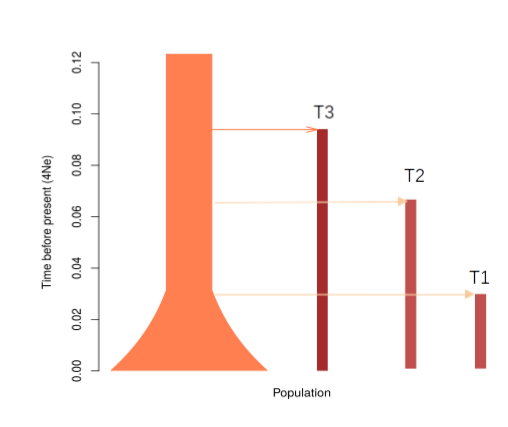
\includegraphics[width=1.00\textwidth]{fig/populations.png}
\decoRule
\caption{\textbf{Demographic models used as simulation scenario.} The y-axis is the time before present and time 0.00 correspond to the time when the sequence data is reported. The time is in units of 4Ne, where Ne represent the effective population size. Initially (time 0.12) there is only one ancestral population. After a number of generations the ancestral population splits in two populations evolving in isolation. I considered three possible times of separation (T1-3). The expectation is that the highest is the separation time the highest is the genetic distance between the two populations measured as $F\textsubscript{st}$.} 
\label{fig:population.pdf}
\end{figure}

\subsubsection{Sequence data simulation using \textbf{ms}}
%ref piu' recenti 
\textbf{ms} \cite{hudson2004ms} is a software that generates sequence samples under a variety of neutral models, allowing one to investigate the statistical properties of such samples, to evaluate estimators or statistical tests, and generally to aid in the interpretation of polymorphic data sets. The program ms can be used to generate many independent replicate samples under a variety of assumptions about migration, recombination rate and population size.\\ 

Using ms, for each scenario I simulated 100 replicates of a 10kb sequence for eighty individuals in two populations (forty each). When considering a population split time of 5k generations ago (T1) I used the following command line: 
\begin{verbatim}
ms 80 100 -T -t 11.2 -I 2 40 40 -g 1 44.36 -n 2 0.05 -eg 0.03125 1 0.0 -ej 0.03125 2 1   
\end{verbatim}

The explanation of the parameters used by ms is the following:

\begin{itemize}
\item\textbf{nsam<nsample>:} this is the first number after the command ms and it is the number of sequences of the locus in each replicate; 

\item\textbf{nrep<nreplicate>:} this is the second number after the command ms and it is the number of independent replicates to generate;

\item\textbf{t <mutationrate>:}
is equal to $$4N0\mu$$ where N0 is the diploid population size and where u is the neutral mutation rate for the entire locus;

\item\textbf{I <individual>:}
followed by the number of subpopulations,npop, and the sample configuration. The sample configuration is a list of npop integers (n 1 n 2...) indicating the number of chromosomes sampled from each subpopulation;

\item\textbf{g <growth>:}
 it indicate the growth of pop1 at a definite time;

\item\textbf{n:}
it set growth of population 2 at time; 

\item\textbf{eg <growth rate>:}
pop1 stop growing at time 0.03125;

\item\textbf{ej <join>:}
Pop1 join with pop2. It is the parameter that change in three command. 
\end{itemize}

To simulate the T2 and the T3 parameters the difference in the command line is in the ej parameter that is 0.0625 and 0.0937, respectively. For each scenario I simulated 100 replicates of forty individuals per population for two populations. The output of ms is a file with data on the variable sites for each individual for each population for each replicate. 

%FIGURA FRASE TRE TEMPI SIMULAZIONI 

\subsubsection{Conversion of simulated data in the GFA format}  

To be processed by \vgp, the simulated data must be converted in the GFA format. We did this in two steps. First we transformed the data on variable sites obtained by ms into sequences using Seq-Gen \cite{rambaut1997seq}, than we transformed sequences into graphs with a utility function that I developed, named \textit{seqgen2gfa+vcf}. \\

%I needed the whole sequence rebuilt and the links between the bubbles """SPIEGARE PERCHE', per usare odgi"g


%I convert mstogfa but I need the information about the links between the bubbles. 


While ms provides information on variable sites it does not provide information on the invariable sequence between variable sites, that is necessary to build a graph. I obtained the information on invariable sites exploiting the tree connecting the simulated sequences that is also an output of ms. A tree is an entity that describes relationships between objects (Figure \ref{fig:phylogenies.jpg}). The tips of the tree are called leaves; leaves are connected by branches, whose length is proportional to the observed differences between the leaves; the coalescence of two branches generates a node or vertex. In our case the leaves represent the simulated sequences that we are actually interested in because they represent the individuals at current time. The nodes indicate the most common ancestor of sequences, the root of the tree is a special node located at the beginning of the tree. \\


\begin{figure}[H]
\centering
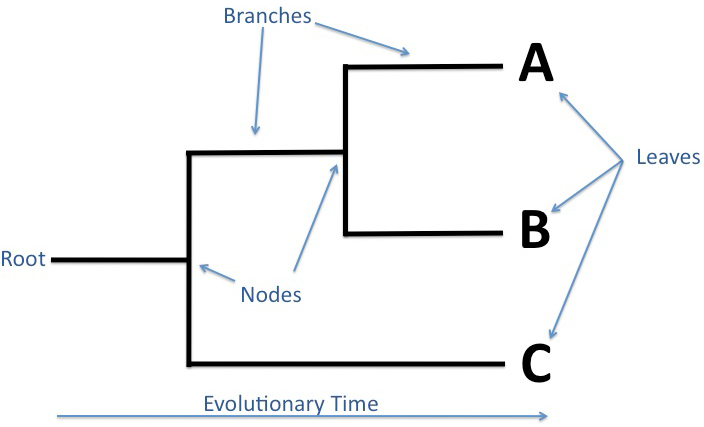
\includegraphics[width=0.70\textwidth]{fig/phylogenies.jpg}
\decoRule
\caption{The crucial components of a phylogenetic tree are nodes, branches, leaves, and the root." \textit{Adapted from} \cite{phylogenetictree}"} 
\label{fig:phylogenies.jpg}
\end{figure}

Seq-Gen \cite{rambaut1997seq} is a program that simulates the evolution of nucleotide sequences along a phylogeny, using common models of the substitution process. A range of models of molecular evolution are implemented, including the general reversible model. 

Using the tree obtained by ms, Seq-Gen reconstructed the entire sequences, including the invariable parts, for all replicates under the three simulated scenario. The command lines for Seq-Gen are: 

\begin{verbatim}
seq-gen -mHKY -l 1000 -s .2 -wa -z 783763255346462154 <treems40popT1> T1.seqgen
\end{verbatim}
where T1.seqgen is the output of the simulations under the scenario T1.
The explanation of the parameters is:

\begin{itemize}
\item\textbf{m <MODEL>:} This option sets the model of nucleotide or amino acid substitution.
\item\textbf{l <SEQUENCELENGTH>:} This option allows the user to set the length in nucleotides or amino acids that each simulated sequence should be.
\item\textbf{s <SCALE>:} This option allows the user to set a value with which to scale the branch lengths in order to make them equal the expected number of substitutions per site for each branch. Basically Seq-Gen multiplies each branch length by this value.
\item\textbf{z <RANDOMNUMBERSEED>:} This option allows the user to specify a seed for the random number generator. Using the same seed (with the same input) will result in identical simulated datasets. This is useful because you can then delete the (often large) simulated sequence files to save disk space. To recreate a set of simulations, you must use exactly the same model options. The default is to obtain a seed from the system clock which will be displayed on the screen allowing it noted down.
\item\textbf{wa:}
Write Ancestral Sequences. This option allows the user to obtain the sequences for each of the internal nodes in the tree obtained with ms \end{itemize}

Once I obtained the variable sites from ms and the sequence from SeqGen I used the \vgpop function \textit{seqgen2gfa+vcf} that I wrote, to convert the sequences from SeqGen to GFA format.  



%-------------------------------------------------------------
\subsection{Calculation of  $F\textsubscript{st}$ from simulated data using \vgp}

I calculated $F\textsubscript{st}$ from the pangenome of the simulated data using the \vgpop function \textit{gfa2vcf}. As a control the simulated sequences were also converted in a VCF file that was used to calculate $F\textsubscript{st}$ with an already existing software: in this way I can compare if the $F\textsubscript{st}$ obtained by the software I wrote are in the same range of those obtained in a different way (Figure \ref{fig:pipeline.pdf}). \\


%cambiare figura 11 in minipresentazione= line1
\begin{figure}[H]
\centering
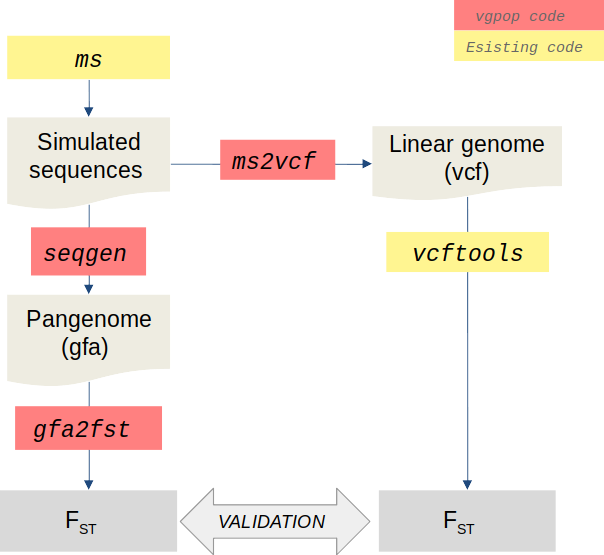
\includegraphics[width=1.00\textwidth]{fig/pipeline.png}
\decoRule
\caption{\textbf{Pipeline for the application and validation of \vgp to simulated data.} I used the software ms to produce 100 replicates of simulated variable sites in a 10kb region for eighty individuals under each of the three scenario in Figure \ref{fig:population.pdf}. The variable sites were transformed in sequences that include also the invariable part using SeqGen and the sequences were used to reconstruct the pangenome of the simulated data that was then processed with the \textit{gfa2fst} function of the \vgp library. $F\textsubscript{st}$ calculation was validated using a software, vcftools, that uses a different $F\textsubscript{st}$ formula. }
\label{fig:pipeline.pdf}
\end{figure}

\begin{figure}[H]
\centering
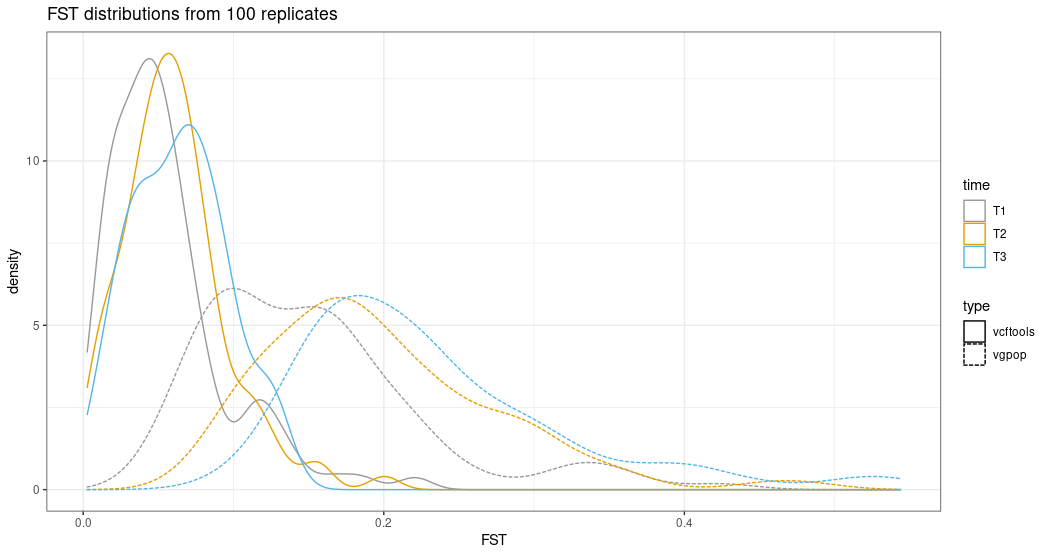
\includegraphics[width=1.00\textwidth]{fig/Fstvcftoolsandvgpop.png}
\decoRule
\caption{\textbf{Application of \vgp to simulated data.} Distributions of the $F\textsubscript{st}$ form 100 replicates of each scenario in Figure \ref{fig:population.pdf}. One set of values (continuous line) is obtained using \vgpop, the other (dashed line) is obtained using  vcftools.  }
\label{fig:fsttime.png}
\end{figure}


$F\textsubscript{st}$ was calculated for each replicates of each scenario. Figure \ref{fig:fsttime.png} shows the distributions of $F\textsubscript{st}$ relative to the three scenario and Table \ref{fig:fsttime.png} reports the relative summary statistics. The first observation form the results is that the $F\textsubscript{st}$ trend vary according to expectation of the three simulated scenario, i.e. the lowest value is found at T2 and the highest at T3. I observe the same trend when calculating $F\textsubscript{st}$ with a different formula as a control. Nevertheless the overall values of $F\textsubscript{st}$ obtained from \vgp are lower that those obtained from vcftools, suggesting that a further comparison would be required to fully clarify the discordance and that there is room for improvement of the \vgp library.  
%FRASE CHE COMMENTA I RISULTATI doppo che vediamo la figura definitiva    Fst is the same from GFA and VCF file.\\
 
\begin{figure}[H]
\centering
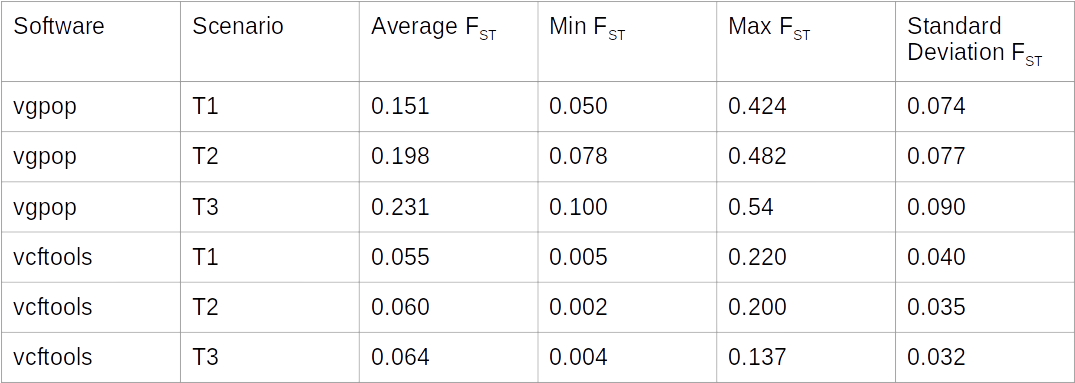
\includegraphics[width=1.00\textwidth]{fig/tabvcftoolsvgpop.png}
\decoRule
\caption{\textbf{Summary statistics of the distributions of the  $F\textsubscript{st}$ }.}
\label{fig:fsttime.png}
\end{figure}



\newpage
\section{Application of \vgp to real data: allele frequencies at variable loci of the HLA region}

HLA is an highly polymorphic region of the genome and it is particularly difficult to assemble with linear methods. The HLA region represent a typical case in which the use of pangenomes can improve the mappability of the sequence reads and the discovery of genomic variants \cite{chin2019diploid}.I considered three genes of the HLA region, \textit{HLA-E}, and \textit{HLA-DMA}, and \textit{HLA-C}.\\

\textit{HLA-E} belongs to non-classical MHC class I (MHC Ib) genes. HLA-E protein shares high structural and functional homology with other MHC class I molecules. \textit{HLA-E} is expressed on most nucleated cells of the human body. However, surface expression of HLA-E protein was found in a restricted set of tissues. In particular, it has been found on leukocytes,endothelium, and cells of the trophoblast\cite{kanevskiy2019dimorphism}.

The protein coded by the MHC class II gene \textit{HLA-DMA} function in the loading of peptides on class II molecules. Like the class II genes, the \textit{HLA-DMA} gene contains upstream regulatory sequences similar to the S-X-Y regulatory region as well as additional putative regulatory sites \cite{westerheide1997hla}.
%The MHC class II homologous  proteins HLA-DMA and HLA-DMB  function in the loading of peptides  onto class II molecules. like the class II genes, the HLA-DM genes contain  upstream  regulatory sequences similar  to  the S-X-Y regulatory  region as well as additional putative regulatory sites.\cite{westerheide1997hla}

The product of the \textit{HLA-C} gene belongs to the HLA class I heavy chain paralogues. This class I molecule is a heterodimer consisting of a heavy chain and a light chain (beta-2 microglobulin). The heavy chain is anchored in the membrane. Class I molecules play a central role in the immune system by presenting peptides derived from endoplasmic reticulum lumen. They are expressed in nearly all cells\cite{HLA-C}\\

For these three genes I started from eleven (\textit{HLA-DMA}), nine (\textit{HLA-E}), and ten (\textit{HLA-C}) sequences downloaded from GenBank. I used the sequences to reconstruct the pangenomes as described in the methods. The pangenomes of \textit{HLA-E} and \textit{HLA-DMA} are less complex compared to the pangenome of \textit{HLA-C}, suggesting less diversity in these two genes compared to \textit{HLA-C} (Figure \ref{fig:pangenomesHLA.png}).\\ 

\begin{figure}[H]
\centering
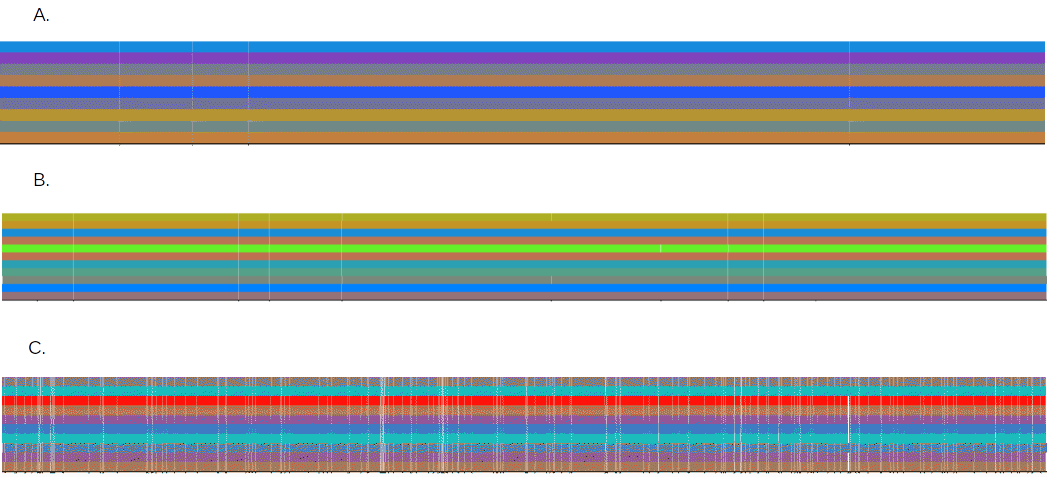
\includegraphics[width=1.00\textwidth]{fig/pangenomes.png}
\decoRule
\caption{\textbf{Pangenomes of the \textit{HLA-E} (A), \textit{HLA-DMA} (B), and \textit{HLA-C} (C) genes.} Colors represent different sequences. Vertical white lines indicate variable sites. Chunks in full color represent invariable region of the sequence}
\label{fig:pangenomesHLA.png}
\end{figure}


Going into more details, in the \textit{HLA-E} pangenome in Figure \ref{fig:hla-e.pdf}A, the first row is the randomly chosen reference sequence while the other rows are the other eight sequences (paths). In the same figure, panels B and C are zoom of two variable sites, i.e. the region of the pangenome for whic I calculated the allele frequencies using the \textit{gfa2allelefreq} function of \vgp. A similar view of the variable sites for the \textit{HLA-DMA} gene is given in Figure \ref{fig:hla-dma.pdf}

This calculation starts with the detection of variable sites (bubbles) with \bbp, and then the allele frequencies are calculated as the number of paths supporting the variant node divided by total number of paths.
In particular, in panel B three sequences have the same allele as the reference, therefore the allele frequency of the reference allele is 3/9=0.66. Similarly, in panel C four sequences have the same allele as the reference, therefore the allele frequency of the reference allele is 0.44. \\

Overall, \textit{gfa2allelefreq} found four variable sites in nine sequences for the HLA-E gene and nine variable sites in eleven sequences for the HLA-DMA gene. The allele frequency values are detailed in Table \ref{tab:gfa2freqandvcf}. \textit{gfa2allelefreq} was not able instead to process the HLA-C pangenome because of its complexity, suggesting  
that an addition to current algorithm is required to handle complex bubbles. %(Figure  una bubble da HLA-E una bubble complessa da HLA-C). 


%Fig: (\ref{fig:pangenome.pdf}A)  for the column in white: first row represent REF, the left node in the REF there isn't in six path, in fact for calculate allele frequencies six paths are divided with 9, the result is 0.66 (\ref{tab:gfa2freqandvcf}first row).

%The same for the second column, left node there aren't in 5 paths, and for calculate allele frequencies I divided 5 paths for the total of paths i.e  9, the result is 0.56.







%aggiungere fig 5.11 bubble per B e C







%and for the first time I calculate \textit{gfa2vcf}, I convert with odgi GFAformat in an odgiformat. I applicate this function and I obtained VCF.

%I build pangenome of HLA (see methods) and for the first time I calculate \textit{gfa2vcf}, I convert with odgi GFAformat in an odgiformat. I applicate this function and I obtained VCF.

%\begin{verbatim}
%odgi build -g E-3133.gfa -o E-3133.og
%\end{verbatim}

%For validate this result I use vg.
%\begin{verbatim}
%vg view -Fv E-3133.gfa > E-3133.vg
%vg index E-3133.vg -x E-3133.xg
%vg deconstruct -p "gi|568815592:30489405-30494204" E-3133.xg
%\end{verbatim}
%The results are the same.



{\small
\begin{table}
\caption{\textbf{Allele frequencies at variable sites within the \textit{HLA-E} and \textit{HLA-DMA} genes.} The column POSITION refers to the position in the pangenome. The variant in position 2844 of the \textit{HLA-DMA} pangenome is a deletion, also represented in Figure \ref{fig:hla-dma.pdf}C} 
\label{tab:gfa2freqandvcf}
\centering
\begin{adjustbox}{width=0.70\textwidth}
\begin{tabular}{c c c c c c}
\toprule
\tabhead {GENE} & \tabhead{PANGENOME} & \tabhead{POSITION} & \tabhead{REF} & \tabhead{ALT} & \tabhead{FREQ} \\
\midrule
\textit{HLA-E} & HLAE-3133 & 551 & T & C & 0.67\\
\textit{HLA-E} & HLAE-3133 & 883 & G & A & 0.56\\
\textit{HLA-E} & HLAE-3133 & 1141 & T & A & 0.11\\
\textit{HLA-E} & HLAE-3133 & 3904 & G & A & 0.67\\
\textit{HLA-DMA} & HLADMA-3108 & 310  & C & T & 0.36\\
\textit{HLA-DMA} & HLADMA-3108 & 3288 & C & G & 0.09\\
\textit{HLA-DMA} & HLADMA-3108 & 2372 & G & A & 0.272\\
\textit{HLA-DMA} & HLADMA-3108 & 3512 & C & T & 0.18\\
\textit{HLA-DMA} & HLADMA-3108 & 3135 & G & A & 0.18\\
\textit{HLA-DMA} & HLADMA-3108 & 1155 & C & T & 0.09\\
\textit{HLA-DMA} & HLADMA-3108 & 1023 & G & A & 0.09\\
\textit{HLA-DMA} & HLADMA-3108 & 2844 & CCT & C & 0.18\\
\textit{HLA-DMA} & HLADMA-3108 & 1468 & A   & G & 0.09\\
\bottomrule\\
\end{tabular}
\end{adjustbox}
\end{table}
}


\begin{figure}[H]
\centering
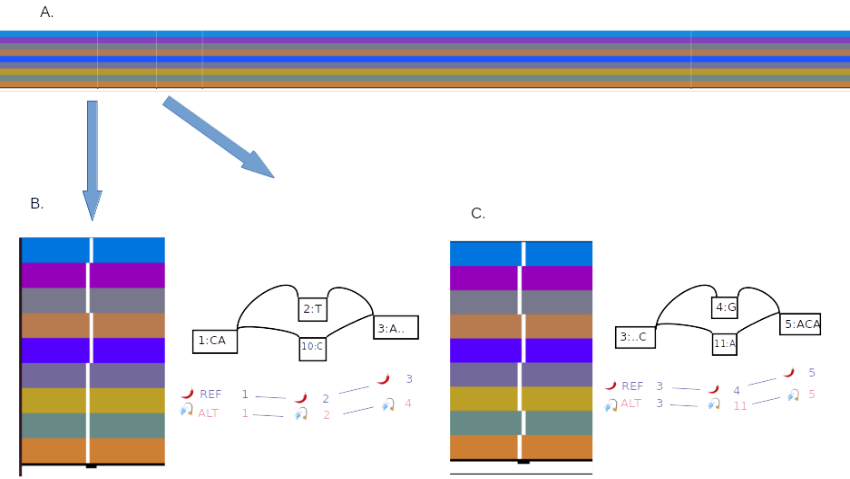
\includegraphics[width=0.80\textwidth]{fig/HLA-E.png}
\decoRule
\caption{\textbf{Variable sites within the pangenome of the \textit{HLA-E} gene obtained from nine sequences.} Panel \textbf{A} shows the whole gene length, while panels \textbf{B} and \textbf{C} are zooms of two variable sites. In the linear representations each line is a sequence, the top one being the randomly chosen reference. Chunks in full color represent invariable parts of the genome while white vertical rows represent variable sites. In panels \textbf{B} and \textbf{C} variable sites are also represented as graphs with paths.}
\label{fig:hla-e.pdf}
\end{figure}



\begin{figure}[H]
\centering
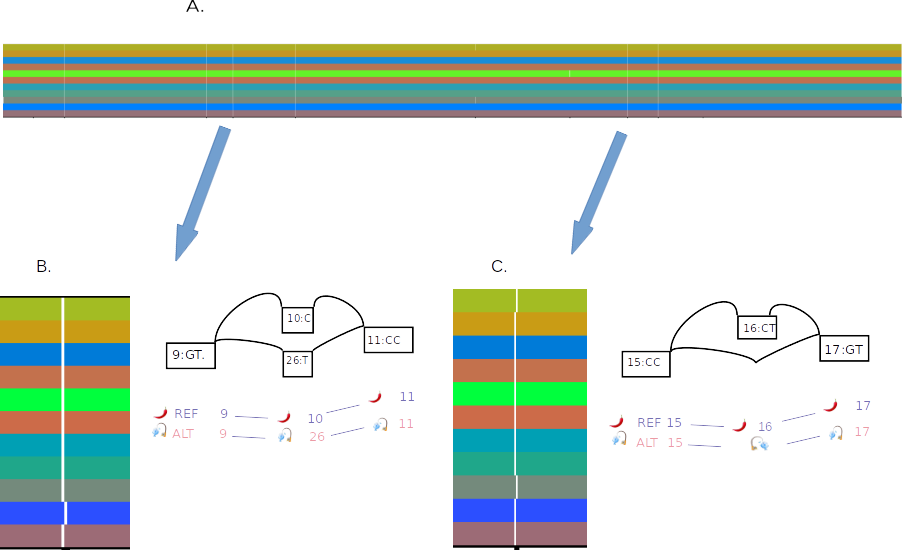
\includegraphics[width=0.80\textwidth]{fig/HLA-DMA.png}
\decoRule
\caption{\textbf{Variable sites within the pangenome of the \textit{HLA-DMA} gene obtained from nine sequences.} Same scheme as in Figure \ref{fig:hla-e.pdf}. The variant detailed in panel \textbf{C} is a deletion.}
\label{fig:hla-dma.pdf}
\end{figure}






%colonna gene, chr diventa pangenome HLA-E, HLA-DMA

